\begin{figure}[htb!]
  \begin{center}
    \resizebox{\textwidth}{!}{
      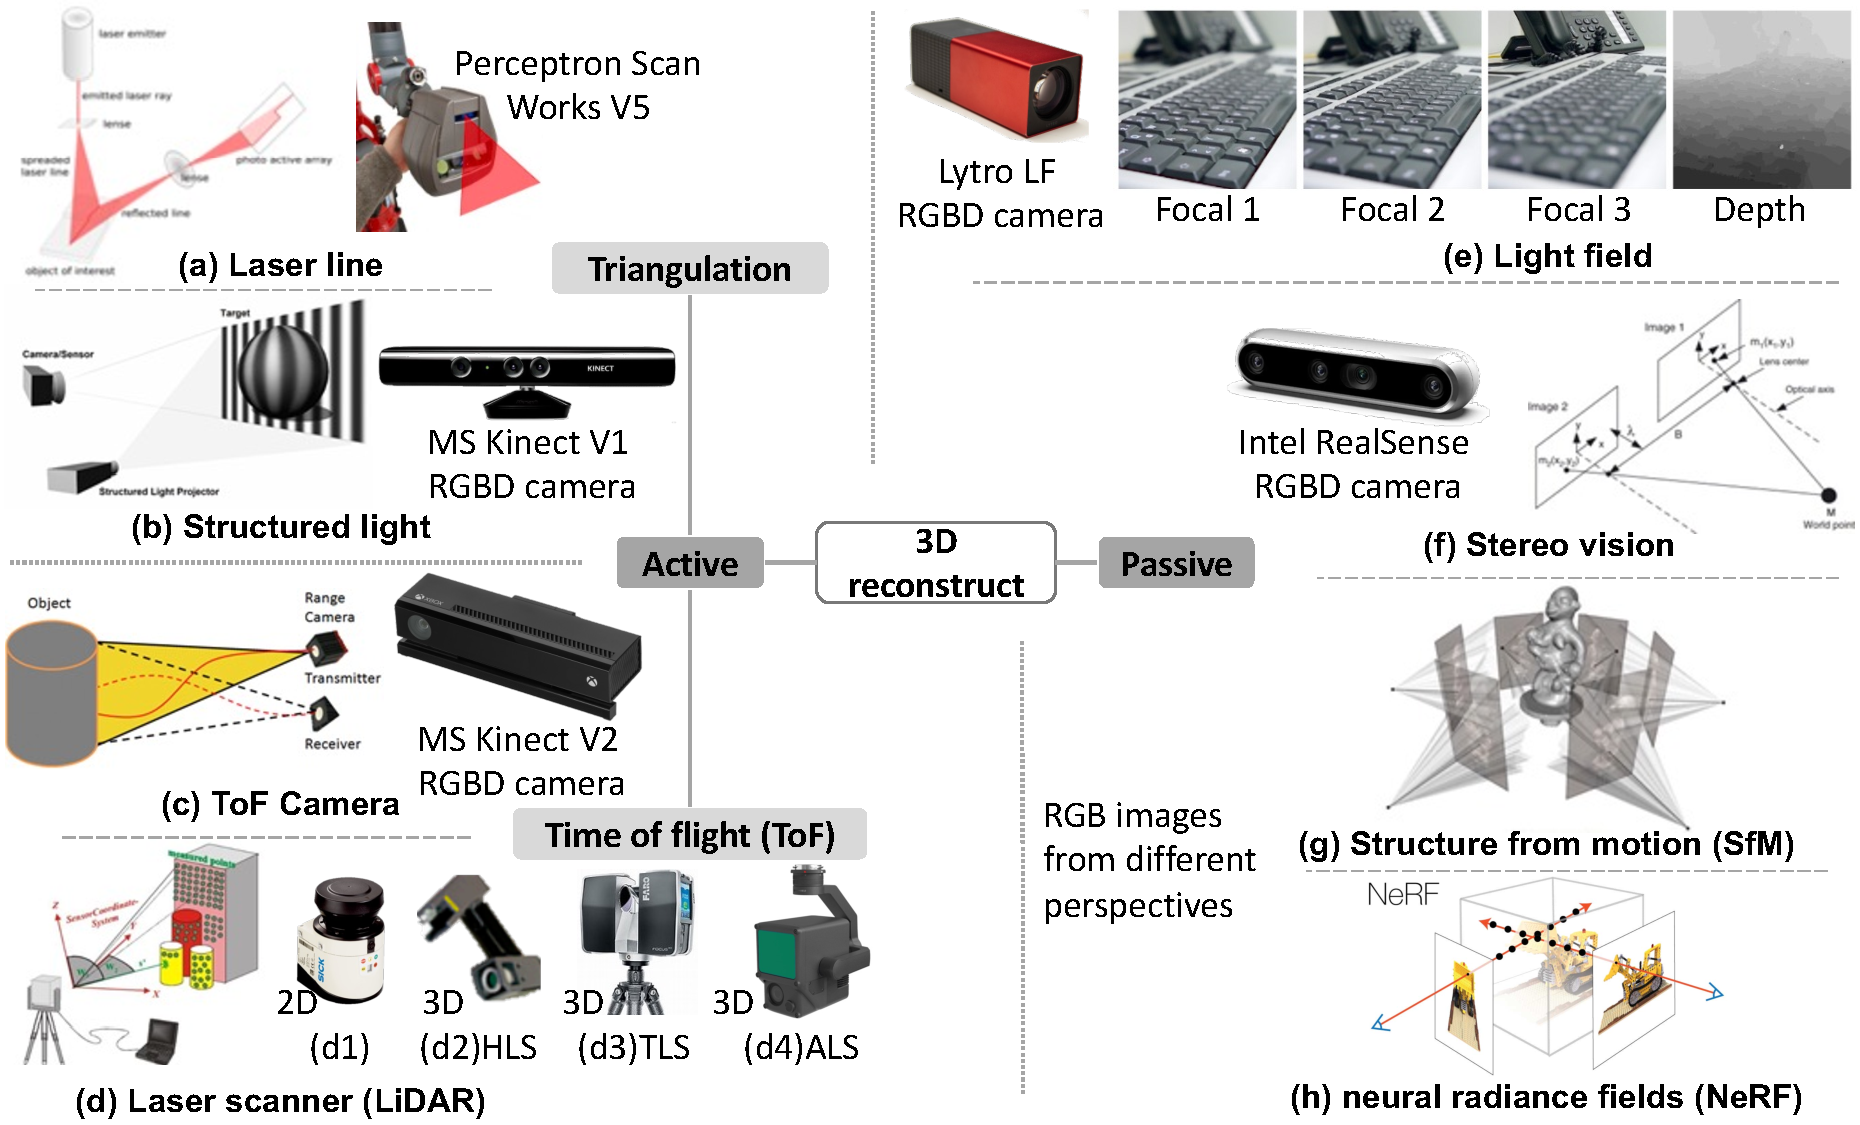
\includegraphics{figures/int/recons_sensors.pdf}
    }
  \end{center}
  \caption[Common approaches for 3D structure reconstruction]{
    Common approaches for 3D structure reconstruction; (a-d) The active sensors rely on projecting lights on the object and analyzing the reflection results; (a) the theory of laser line \citep[Fig.~1]{zhou_real-time_2020} and one commercial device used by \citet[Fig.~2]{schunck_pheno4d_2021}; (b) the theory of structured light \citep[Fig.~4]{paturkar_making_2021} and one commercial device \citep[Fig.~1]{duc_combined_2015}; (c) The theory of \gls{tof} camera \citep[Fig.~2.1]{jamtsho_geometric_2010} and one commercial device (\url{https://en.wikipedia.org/wiki/Kinect}); (d) the theory of \acrfull{lidar} \citep[Fig.~4]{khomsin_analysis_2019}; (d1) 2D lidar scanner (\url{https://www.sick.com/de/en/lidar-sensors/2d-lidar-sensors/lms1xx/c/g91901}) (d2) \acrfull{hls} \citep[Fig.~2b]{ameen_evaluation_2018}; (d3) \acrfull{tls} (\url{https://downloads.faro.com/index.php/s/89t7CjYKcjGZd3R} Fig.~1-1); (d4) \acrfull{als} (\url{https://enterprise.dji.com/zenmuse-l1}); (e-f) the passive sensors rely on analyzing the passively received image groups; (e) one commercial light field camera and its collected data \citep[Fig.~1\&6]{schima_imagine_2016}; (f) the theory of stereo vision \citep[Fig.~1]{kim_3d_2003} and one commercial device (\url{https://www.intelrealsense.com/depth-camera-d455}) (g-h) the \gls{rgb}-based 3D reconstruction algorithms from several perspective images, via (g) conventional geometric deduction \citep[Fig.~6]{shalma_review_2023} and (h) deep learning (\url{https://www.matthewtancik.com/nerf})
  }
  \label{fig:int2}
\end{figure}